\documentclass[11pt,english]{article}
\usepackage[latin9]{inputenc}
\usepackage[letterpaper]{geometry}
\geometry{verbose,tmargin=1in,bmargin=1in,lmargin=1in,rmargin=1in}
\usepackage{babel}
\usepackage{amsmath}
\usepackage{amssymb}
\usepackage{capt-of}
\usepackage{graphicx}
\usepackage[usenames,dvipsnames]{color}
\usepackage{latexsym}
\usepackage{xspace}
\usepackage{pdflscape}
\usepackage[hyphens]{url}
\usepackage[colorlinks]{hyperref}
\usepackage{enumerate}
\usepackage{ifthen}
\usepackage{float}
\usepackage{placeins}
\usepackage{array}
\usepackage{tikz}
\usetikzlibrary{shapes}
\usepackage{algorithm2e}
\setcounter{MaxMatrixCols}{20}

\newcommand{\rthree}{\mathbb{R}^3}
\title{CIS 521 Homework 6 \\
Due:  Tuesday March 29th}
 \author{Gabrielle Merritt}
 
\date{}

\begin{document}
\maketitle
\begin{abstract}
This spam filter built on the original spam filter from Homework 5, in which I created a simple naive bayes spam filter that tokenized email bodies and predicted probabilities of word occurance in spam and ham emails, to train a spam and ham classifer. With the improved spam classifier I used bigrams instead of unigrams as well as  tokenized more than just the body of the email.
\end{abstract}
\section*{System Design} 

For the system design I used the same basic outline as the previous homework, which is a spam filter class, that takes in the paths to the spam and ham training data, and calls a function that tokenizes and calculates the log probabilities for all of the emails in the training path. I also hard code a smoothing constant for all spam filter classes. Most of the changes made to gain a higher accuracy on this assignment were made in the pre processing and tokenization functions called in the inialization function. 
\section*{Features}
The main features I expiramented with were, the smoothing parameter, bigrams, tokenization, and punctuation. 
I implemented a function to calculate the bigram probabilities, as well as functions that read in the entire email, instead of just the body of the email.
To calculate the birgram probabilities I used 
After experiencing some progress with implementing these features, I used python's regex package in order to split punctuation from words and count them as seperate tokens. With these features implemented I was able to obtain a 99 percent total accuracy rate without changing the smoothing parameter. 
\section*{Results}
\begin{figure}[h!]
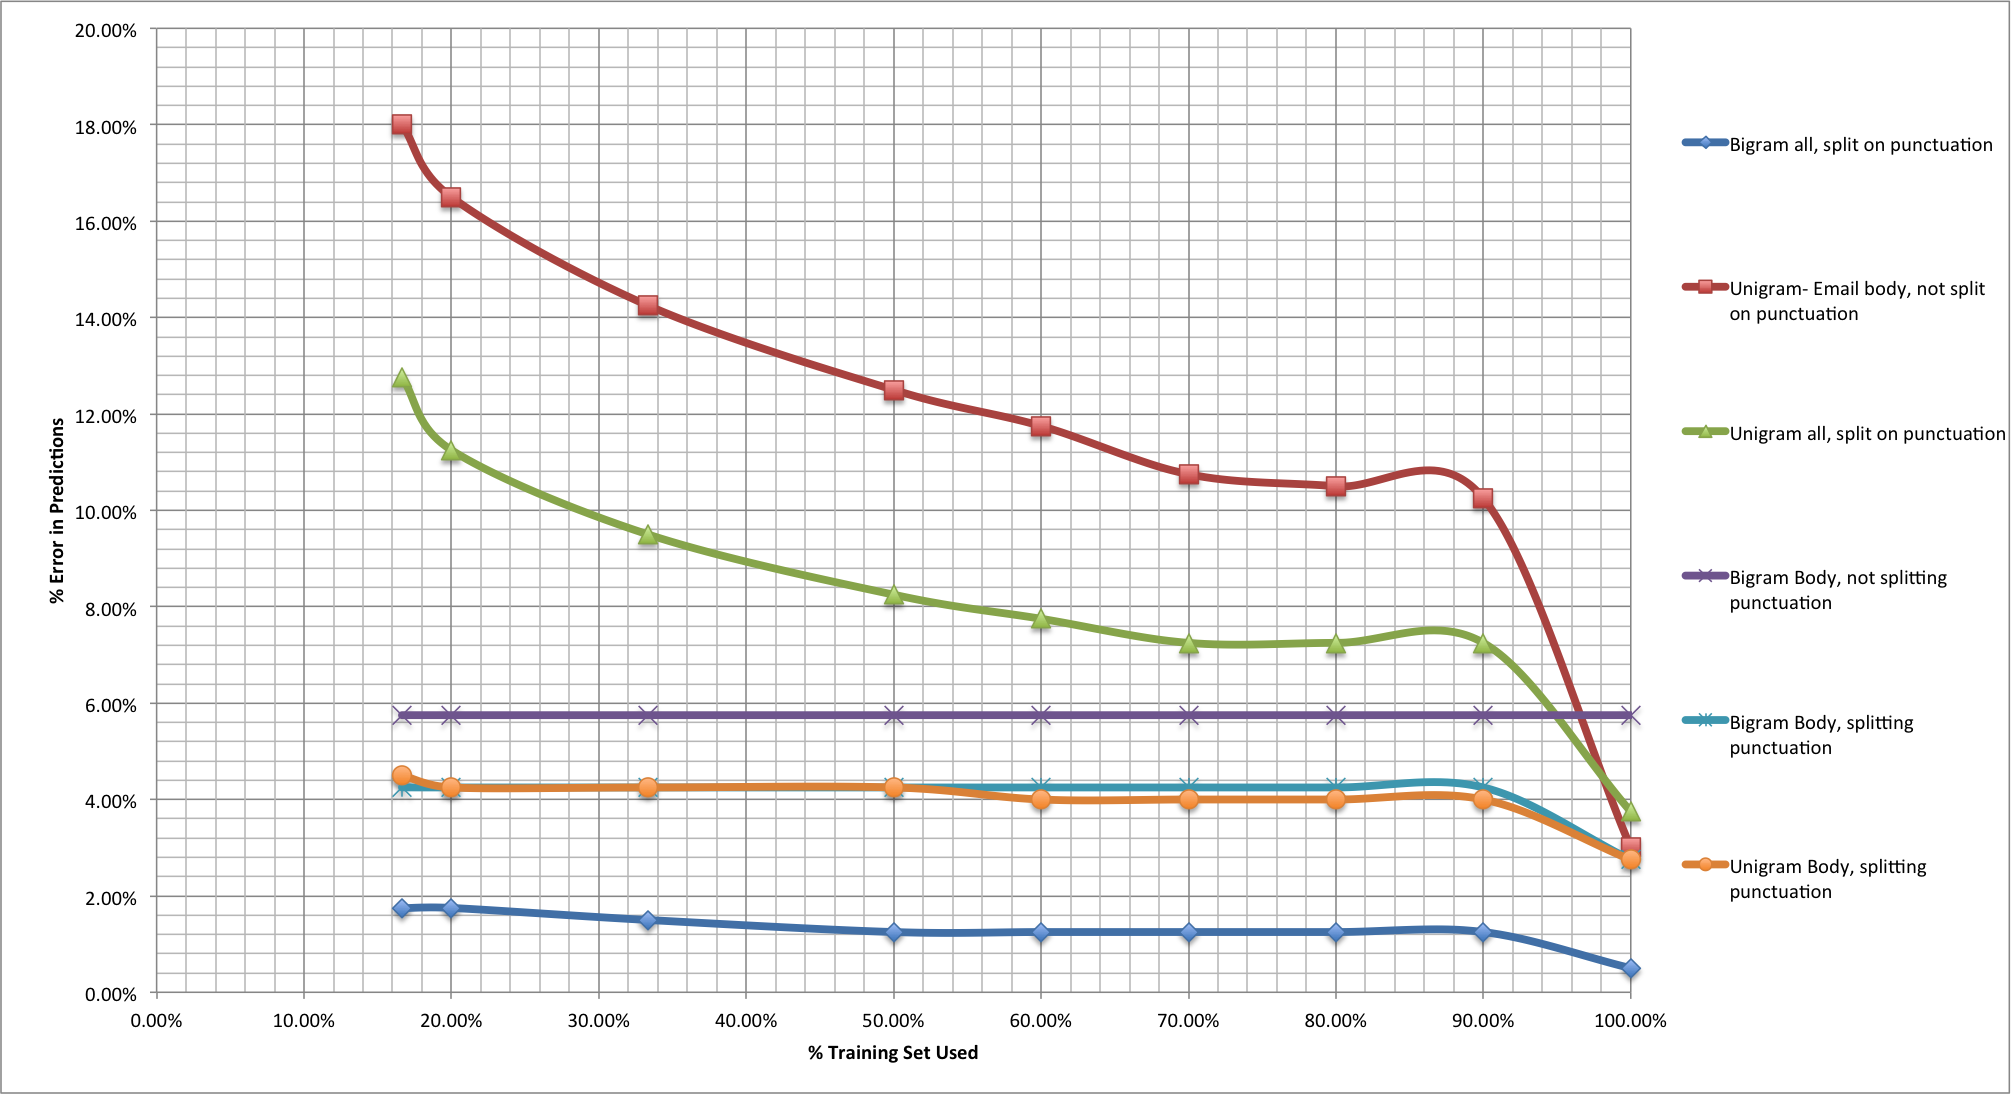
\includegraphics[width = \linewidth]{chrt.png}
 \caption{ Blue line - Bigram splitting on punctuation, and using entire email} 
\end{figure}
\FloatBarrier
To test the validity of my results, I decided to compare how my classifer behaves only using a subset of the training data. I compared my original classifier (Unigram, Email Body only, No split on punctuation) as well as variations of Bigram, using the entire email or just the body, and splitting on punctuation.  From the data it seems that in general using Bigram gives much more stable results than using only unigrams, their prediction error isn't as subseptible to poor training. However, using punctuation as tokens (splitting on punctuation) seems to yield better performance in general. The blue line on the graph is my final classifier model, which uses the entire email, splits on punctuation and uses bigram probabilities.  
\linebreak
	For the test data given and restricting the smoothing constant to $1^{-100}$, I am able to correctly classify all but one email (ham/dev118). After slowly increasing the smoothing constant to see what other emails with a much larger constant are mis-classified, it seems that language in the body of ham/dev118 is what trips up my classifier. From what I can see most of the ham emails / training emails don't usually include language  like "compare", "As of today". Additionally mailers with addresses like @spamassassin tend to be labelled as spam by my classifier, according to my indicitive of spam function. When I checked the maximum likelyhood values for ham or spam for that specific email i noticed the values $ ham = -4042.04065163 $ and $spam = -3975.75497737$ are realitively close in value, so perhaps adding more features to my classifier could help. 

\end{document}
